\chapter{Anhang}


\section{Quellcodeauszug}
Im der Abbildung \ref{aircraftFamilySelectionViewModelClass} ist das vollständige ViewModel für die Auswahl des Flugzeugprogramms zu sehen. Die Klasse wurde für ein Beispiel der Navigation in der Anwendung verwendet und ist im Text referenziert.

\begin{lstlisting}[caption=Vollständige SelectAircraftFamilyViewModel Klasse für die Flugzeugprogrammauswahl]
/// <summary>
    /// This View Model has the logic for aircraft family selection. Normally its the first view if
    /// a new configuration is started.
    /// </summary>
    public class SelectAircraftFamilyViewModel : GridHolderViewModel
    {
        private AircraftModel _model;
        private ICommand _familySelectedCommand;

        public SelectAircraftFamilyViewModel()
        {
            _model = new AircraftModel();
            InitializeDataSource();
        }

        private void InitializeDataSource()
        {

            DataGroupElements = new ObservableCollection<DataCommon>
                {new AircraftProgrammGroup(_model.GetAllAircraftProgramms())}; 
        }
        public ICommand SelectAircraftCommand
        {
            get { return _familySelectedCommand ?? (_familySelectedCommand = new RelayCommand<DataCommon>(SaveSelectionAndNavigateToSummaryPage)); }
            set
            {
                _familySelectedCommand = value;
                OnPropertyChanged();
            }
        }

        private void SaveSelectionAndNavigateToSummaryPage(DataCommon data)
        {
            var selectedProgramm = GetSelectedProgramm(data.UniqueId);
            _model.SelectAircraftProgramm(selectedProgramm);
            var classToNavigate = SimpleIoc.Default.GetInstance<ISummary>();
            var navigationService = SimpleIoc.Default.GetInstance<INavigationService>();
            navigationService.Navigate(classToNavigate.GetType());
        }

        private AircraftProgramm GetSelectedProgramm(string uniqueId)
        {
            return _model.GetAllAircraftProgramms().FirstOrDefault(programm => programm.UniqueId.Equals(uniqueId));
        }
    }
\end{lstlisting} 
\label{aircraftFamilySelectionViewModelClass}

 
\section{Evaluationsergebnisse} \label{anhangEva}
Im Folgenden werden die kompletten Ergebnisse der Evaluation dargestellt. Die Fragebögen für die Experten (siehe \ref{evaluationBogenExpert}) und der Benutzer (siehe \ref{evaluationSheetUser)


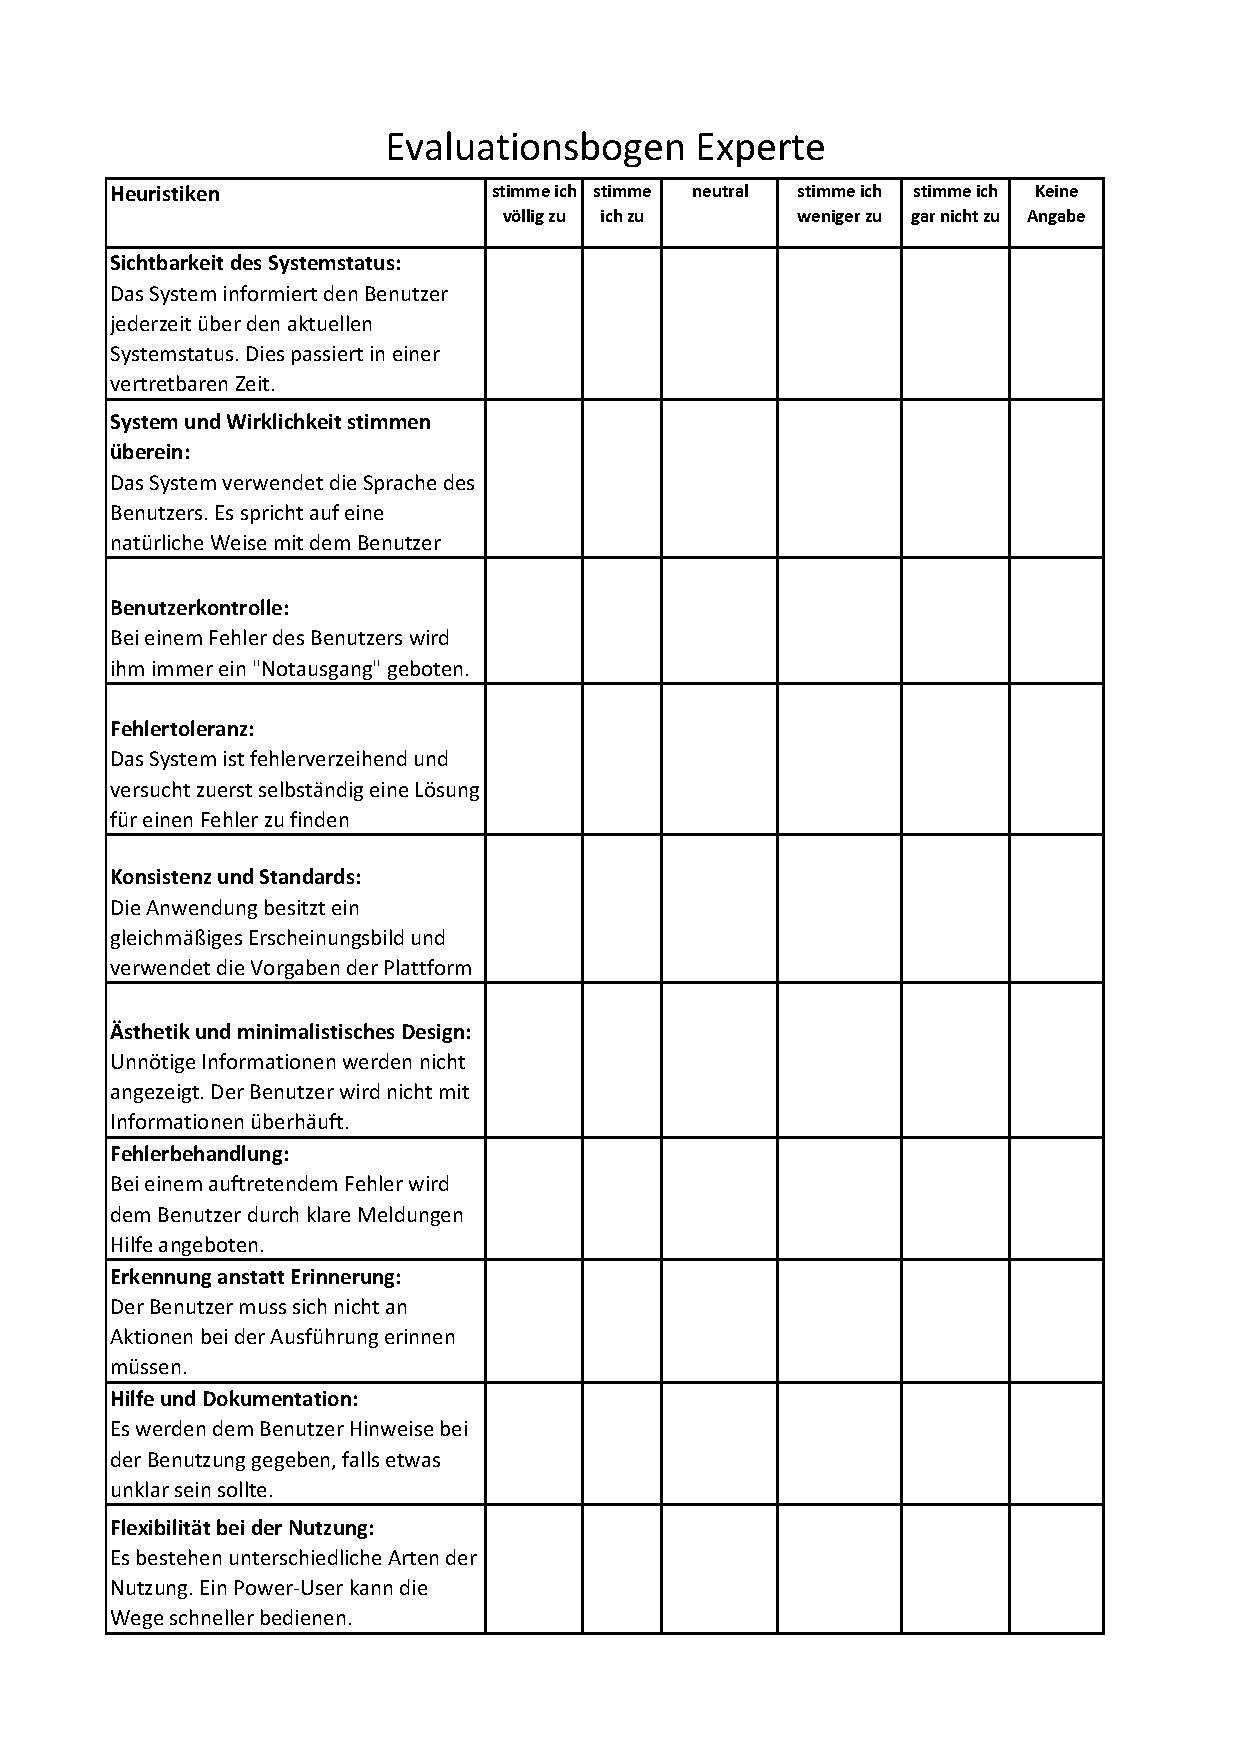
\includepdf[pages=1]{anhang/evaluationsbogenExperte.pdf}
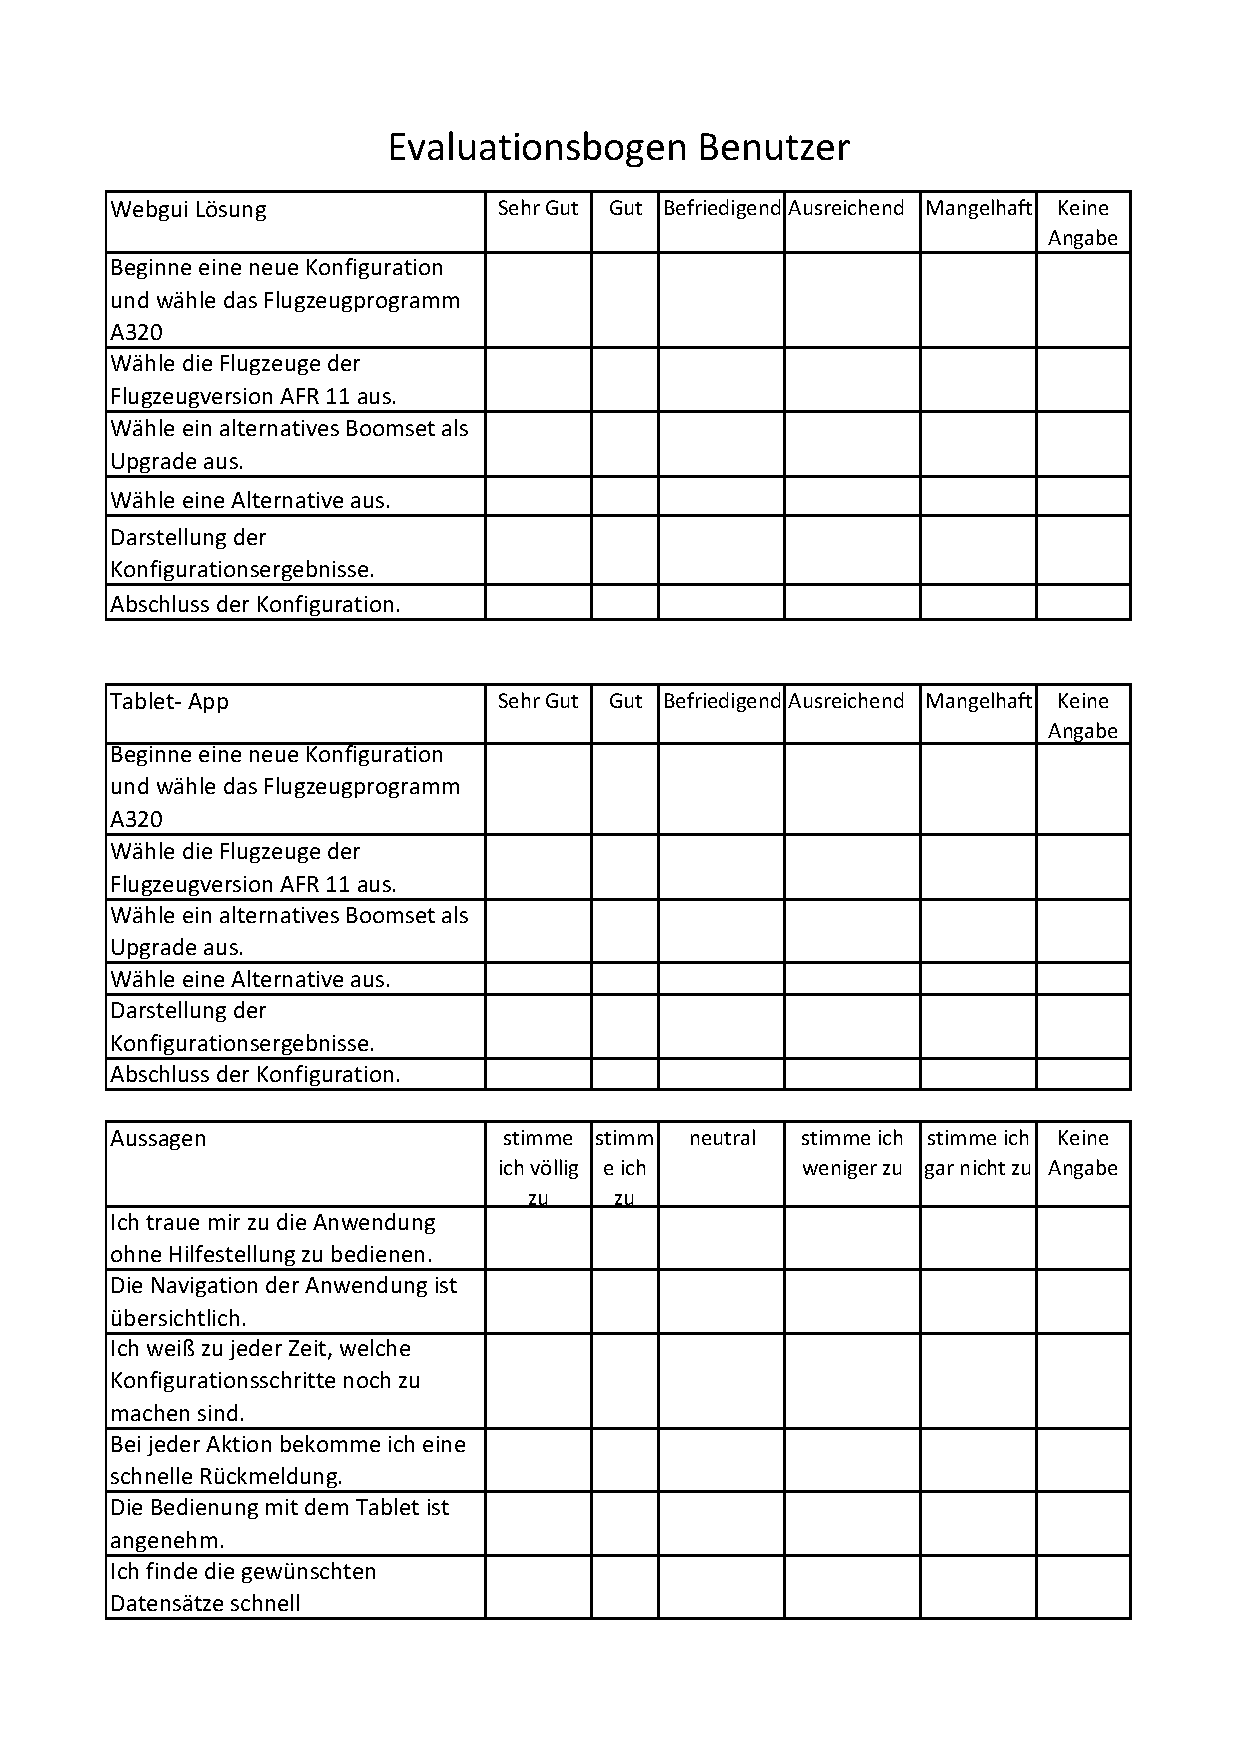
\includepdf[pages=1-2]{anhang/evaluationsbogenUser.pdf}
